\normaltrue \difficilefalse \tdifficilefalse
\correctionfalse

%\UPSTIidClasse{11} % 11 sup, 12 spé
%\newcommand{\UPSTIidClasse}{12}

\subsection*{Robot colossus $\star$ \label{C2:06:92}}
\marginnote{\textit{Banque PT -- SIC 2023.}}
\marginnote{\UPSTIcompetence[2]{C2-06}}
\marginnote{\UPSTIcompetence[2]{A3-05}}
\setcounter{question}{0}

\index{Compétence C2-06}
\index{Colossus}

%\index{Train d'engrenages simple}
\ifcorrection
\else
\marginnote{\textbf{Pas de corrigé pour cet exercice.}}
\fi

\ifprof
\else


\begin{marginfigure}
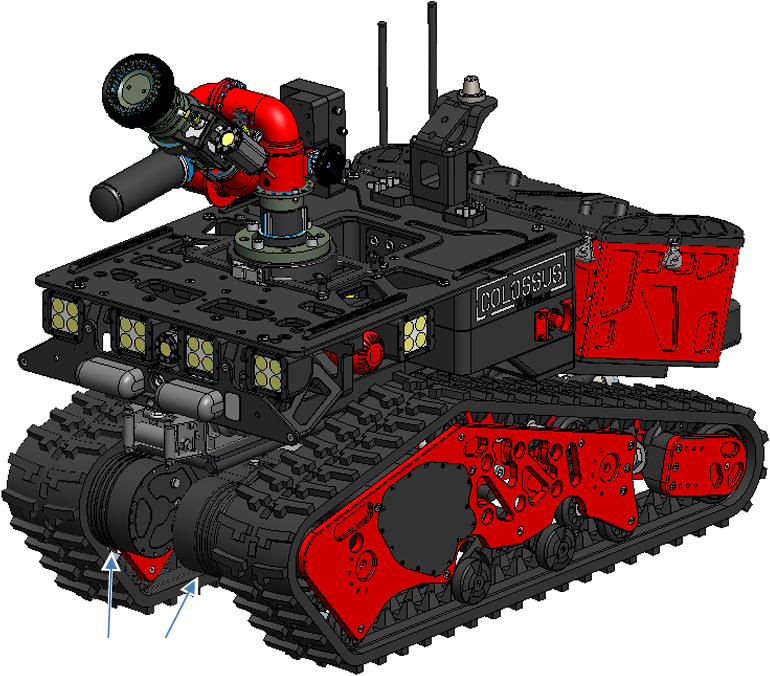
\includegraphics[width=\linewidth]{92_00}
\end{marginfigure}
On s'intéresse à la transmission du robot colossus dont le déplacement est réalisé grâce à des chenilles. On appelle barbotin la pièce sur laquelle s'enroulent ces dernières. Le barbortin est de diamètre \SI{250}{mm}.
Le moteur tourne à \SI{4500}{tr/min}.

\begin{marginfigure}
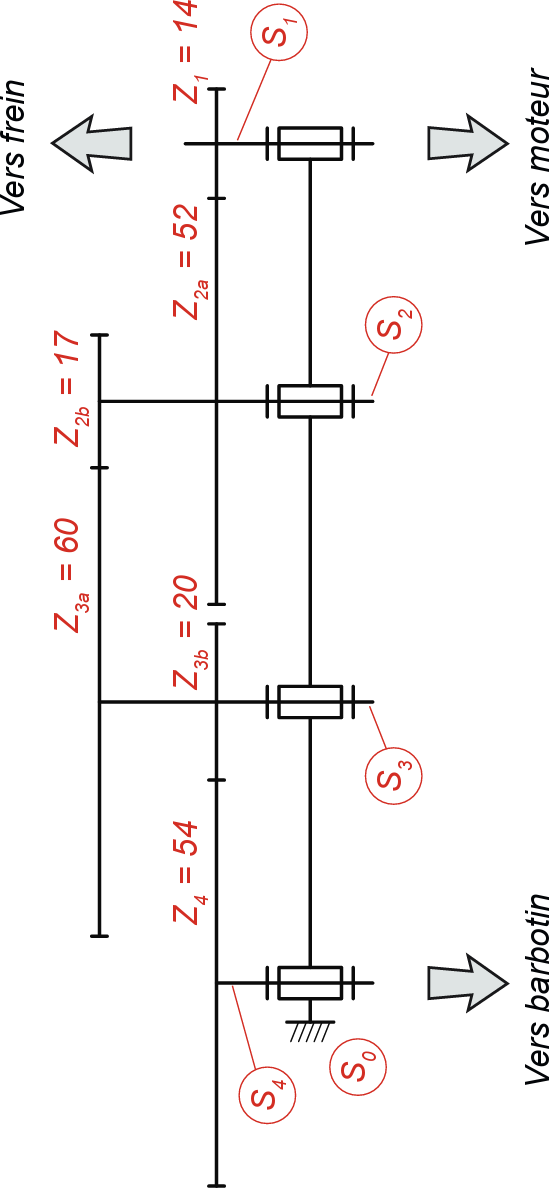
\includegraphics[width=\linewidth]{92_02}
\end{marginfigure}

\begin{center}
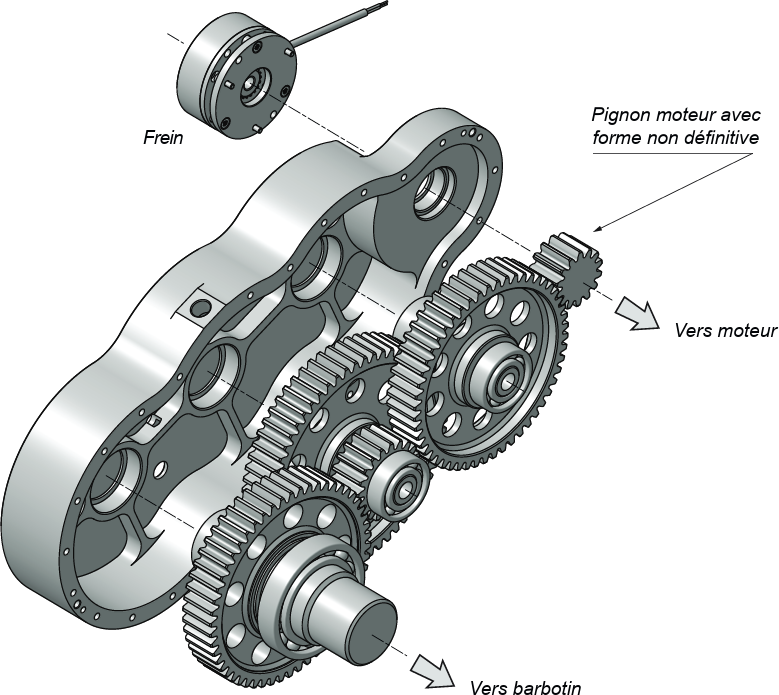
\includegraphics[width=\linewidth]{92_01}
\end{center}


\fi




\question{Donner l’expression littérale du rapport des vitesses $\omega_{4/0}/\omega_{1/0}$ en fonction des différents nombres de dents notés $Z_i$.}
\ifprof
\begin{corrige}
$\dfrac{\omega_{4/0}}{\omega_{1/0}}  = - \dfrac{Z_1 Z_{2b}Z_{3b}}{Z_{2a}Z_{3a}Z_{4}}$.

\textit{AN :} $\dfrac{\omega_{4/0}}{\omega_{1/0}}  = - \dfrac{14\times  17 \times 20}{52 \times 60 \times 54}$ $= - 0,028$.
\end{corrige}
\else
\fi




\question{Déterminer la vitesse du robot.}
\ifprof
\begin{corrige}
Soit $V$ la vitesse du robot, on a donc $V = \omega_{4/0} \dfrac{D}{2}$.

On a donc $V = - \dfrac{Z_1 Z_{2b}Z_{3b}}{Z_{2a}Z_{3a}Z_{4}}  \dfrac{D}{2} \omega_{1/0}$.

\textit{AN :} $V = 0,028 \times 125 \times 4500\dfrac{2\pi}{60}$ $=\SI{1663}{mm.s^{-1}}$. 
\end{corrige}
\else
\fi





\ifprof
\else
\begin{flushright}
\footnotesize{Corrigé  voir \ref{C2:06:92}.}
\end{flushright}%
\fi